\epigraph{\textit{"Why nobody tried to fix this bug?"}}

\paragraph{Abstract} The route to a reliable and efficient device is inevitably a long iterative process. In each optimization step a device is fabricated, evaluated, and the design modified for the next step. Part of the evaluation is just a repetitive process which can be automatized without any loss. I will describe the implementation of a current-voltage sweeps acquisition software, this characterization technique is the most frequently used in our group. Additionally I will describe the routines I developed for the data processing and representation, like fittings, integrations and plots.

\paragraph{Publications} The source code of software included in this chapter has been released and can be accessed on \url{https://github.com/ilario/PyPV} and \url{https://github.com/ilario/photophysics-data-processing-R}.

\section{PyPV: An easy Current-Voltage curves acquisition interface}

\epigraph{\textit{"Ok, I finally completed it, by the way, why did you start developing this?"\\"Well, it was just a proof of concept, but it's nice you worked on it"}}


\subsection{Previous software}
\begin{SCfigure}%[!hbtp]%
	\centering
	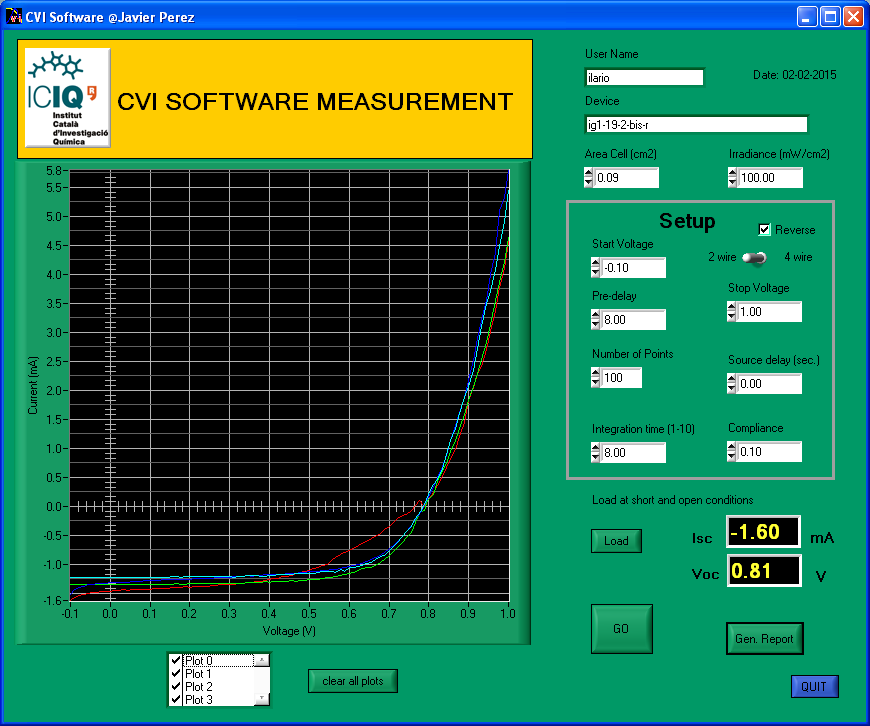
\includegraphics[width=0.5\textwidth]{old_iv_software/old_iv_software.png}
	\caption{}\label{fig:old_iv_software}
\end{SCfigure}

\subsection{Original Project}
I received a proof-of-concept software developed by Daniel Fernandez Pinto and decided to continue the development. At that point the software had an interface with few buttons and a working Keithley communication library.

\subsection{User's requests}

Installation instructions
Shutter control
GPIB GPIB0
\subsection{Implementation and user interface}

\paragraph{Autoscale} As it was explained in \cpageref{autoscale}, the automatic scale setting of the Keithley is detrimental for perovskite solar cells dynamic measurements.

\paragraph{Auto-measure}\label{automeasure}

\paragraph{Resistances} The shunt and series resistances estimation from current-voltage sweeps have been implemented but should not be considered for measurements on hysteretic devices, as explained in \cpageref{resistances}.

\subsection{Limitations}

The interface development has been started with the "Monkey Studio" software, which development has ceased even before the start of PyPV. This demonstrated to be a big failure in long term development planning.

\section{Robust and quick data analysis via R scripts}
\epigraph{\textit{"Is there an Origin version for Linux?"\\"No"}}


\subsection{Charge Extraction (\acr{ce})}\label{r_ce}


\subsection{Transient PhotoVoltage (\acr{tpv})}\label{r_tpv}

\subsection{Transient PhotoCurrent (\acr{tpc})}\label{r_tpc}

\subsection{Differential Capacitance (\acr{dc})}\label{r_dc}

\section{Maximum Power Point Tracking}\label{software_mppt}
\epigraph{\textit{"A student of mine sells a complete system for that, just buy it"}}

CITE Cimaroli2017

http://candlelight-systems.com/
